\documentclass[dvipdfmx]{jsarticle}
\usepackage[T1]{fontenc}
\usepackage[dvipdfmx]{hyperref}
\usepackage{lmodern}
\usepackage{latexsym}
\usepackage{amsfonts}
\usepackage{amssymb}
\usepackage{mathtools}
\usepackage{amsthm}
\usepackage{multirow}
\usepackage{graphicx}
\usepackage{wrapfig}
\usepackage{here}
\usepackage{float}
\usepackage{ascmac}
\usepackage{url}

\title{zoo.csvに関するR言語を使用した決定木構築}
\author{文理学部情報科学科\\5419045 高林 秀}
\date{\today}

\begin{document}

\maketitle

\begin{abstract}
  本稿では、今年度データ科学2で学習した「決定木構築手法」を使用して、本学部ページにて配布されたデータであるzoo.csvの決定木構築を実験するものである。また、決定木構築に際し、分割基準や木の高さなどのパラメータをいくつか変更しながら実験を行う。また得られた決定木の評価指標値として、精度の算出を行い、木の良し悪しを判定する。
\end{abstract}

\section{目的}
本稿では実際に、R言語を使用し配布データであるzoo.csvの決定木構築を行うことで、本年度データ科学2で学習した決定木構築の手法への理解を深め、その定着を図ることを目的とする。また、1年次に学習したlatexを用いたPDF作成の復習も兼ねるものとする。
\section{理論説明}
今回の実験で用いた、計算理論をそれぞれ説明する。
\subsection{分類学習について}
我々の生きている世界には様々なデータが存在する。例えば、農業を行う際「豊作になる条件」を知るには肥料の種類や量、光量や日照時間、温度、雨量等の様々な「属性の値」をもとに予測することが可能である。これを予測する手法として機械学習が挙げられるだろう。機械学習では、コンピュータがある問題とその答えを使用して学習を行い、データに潜むパターン等を識別、発見する技術である。この機械学習は大きく3つに系統が別れている。初めに「教師あり学習」、次に「教師なし学習」、最後に「強化学習」である。そしてそこから更に、求める結果や手法によって「分類」「回帰」「クラスタリング」「次元削減」「Q-Learning」と細かく分割される。中でも、今回扱う「分類」はデータが属するクラスを予測することを目的とする。予測するクラスが2つならば「2値分類」、それ以上ならば「多クラス分類」と呼ばれる。\par
詳細な説明は本稿では行わないが、今回扱う「決定木」は教師あり学習の分類に属する手法である。\par
これまで、分類の手法として「k-近傍法」等を学習してきた。k-近傍法は、最近傍のデータをk個選択し、それらが最も多く属するクラスに識別、分類を行う方法であった。決定木では、k-近傍法の手法とは異なり「木構造」を利用する。ある属性の属性値によってデータを徐々に分割していきクラス分類をする。決定木の詳細については後述する「決定木(Decision tree)」の部分で説明する。\par
なお分類学習には、ここで紹介した手法以外に「サポートベクターマシン(Support Vector Machine:通称SVM)」や 「ナイーブベイズ(Naive Bayes)」などがある。最近ではこれら従来の手法に加え、ニューラルネットワークを利用した手法が画像分類等の分野で広がっている(CNNなど)。
\begin{figure}[H]
  \centering
  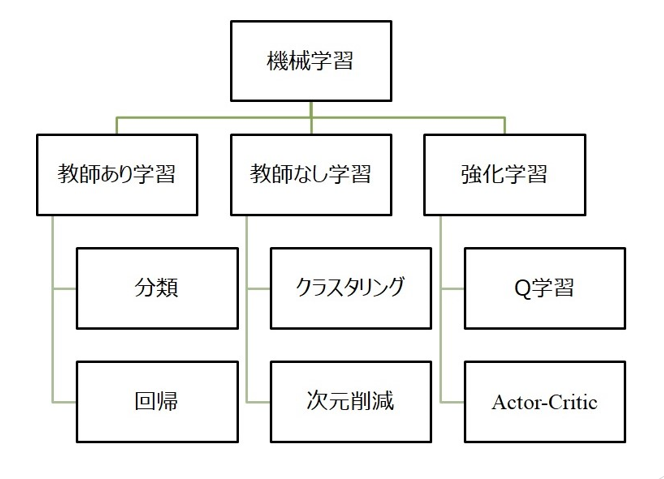
\includegraphics[scale=0.6]{ML.PNG}
  \caption{機械学習の枠組み}
\end{figure}
\subsection{決定木(Decision tree)}
決定木とは「木構造を利用した機械学習手法」である。分類を行う決定木を「分類木」、回帰(連続値の予測)を行う決定木は「回帰木」と呼ばれる。決定木では任意の属性の属性値による条件分岐によって、データを徐々に分割することで結果を出力する。したがって、生成される木構造の枝は分割の結果ラベルを、葉は予測、分類されるクラスの結果を、各ノードは属性に関する分割テスト含んでいる。\par
決定木を使用する例として、ミカンとリンゴを分類する場合を考える。下記の図のように、ミカンの画像を4枚、リンゴの画像を2枚の計6枚の画像データセットがあるとする。
これを、ある条件Aを定め、それに当てはまるもの、そうでないものを分割する。この操作を分割テストという。分割テストの結果によって次の分割テスト行うか否かが決定され、最終的に、ミカンとリンゴが図のように分類される。これが決定木の大まかな流れである。
\begin{figure}[H]
  \centering
  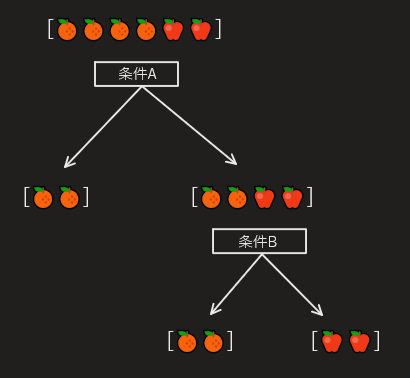
\includegraphics[scale=0.6]{decition_ex1.PNG}
  \caption{ミカンとリンゴの分類木}
\end{figure}
\subsubsection{決定木のメリット・デメリット}
決定木には、前項で述べたSVM等の他の機械学習手法よりも\textbf{分類課程が明確である}というメリットが存在する。これは、分類の結果の理由が他の手法よりも明確である点が挙げられるだろう。例えば先程のミカンとリンゴの例のように条件を満たすか否かによって、データを分割し、ミカンかリンゴか分類する。このとき何故ミカン(またはリンゴ)と分類したのかの理由が「条件A(または条件B)を満たしているから」と容易に説明できるであろう。\par
このように、機械学習を行った結果として生成されるモデルにおいて、判断の仕組みが分かる、説明できるものをホワイトボックス、反対に説明できないあるいは説明しづらいものをブラックボックスと呼ぶ。またホワイトボックスであるようなモデルを備えた人工知能を「説明可能なAI\footnote{説明可能なAI:このように、モデルの解釈性をもたらす研究が近年注目されており、ブラックボックス型のモデルを解釈する手法として「SHAP」「LIME」などがあり、Pythonパッケージが公開されるなど実務での利用が進んでいる。}(XAI:Explainable AI)」と呼ぶ。XAIは米国国防高等研究計画局(DARPA)が手動する研究プロジェクトが発端となった。\par
以下に、決定木のメリット・デメリットをまとめた表を示す。
\begin{table}[H]
  \begin{center}
    \caption{決定木のメリット・デメリット}
    \begin{tabular}{|c|c|} \hline
      メリット & デメリット \\ \hline
      ・学習結果の可読性が高く結果の根拠を説明しやすい & ・条件分岐が複雑になるほど過学習しやすい\\
      ・データの前処理が少なく済むことが多い & ・精度が突出して良いわけではない\\
      ・予測時に必要な計算量が小さい & \\
      ・回帰、分類の両方に対応可能 & \\ \hline
    \end{tabular}
    \label{hyo01}
  \end{center}
\end{table}
なお、下記サイトにおいて説明可能なAIの詳細な記載があるのでそのリンクを示す。\par
\url{https://blog.global.fujitsu.com/jp/2018-12-27/01/} \par
このように決定木は、分類課程が分かりやすいためエキスパートシステム\footnote{エキスパートシステム:ある分野における専門知識を蓄積し、その分野の専門家のように振る舞うことができる。}等に利用されることが多い。\par
決定木は、分割テストに使用する属性によって分割結果が変わることは、容易に想像することができる。データの属するクラスの割合をクラス分布と呼ぶ。決定木の分割テストでは、クラスを分類したいのでデータのクラス分布が偏れば偏るほど良い。しかし、分割テストに使用する属性によってクラス分布が偏ったり、均等になってしまいクラス分布があまり変化しない、といったことが発生する。そこで、分割テストに使用する属性を決定するためにいくつか評価基準が存在する。
\subsection{分割に用いる属性の選択基準}
分割テストに使用される属性は、下記のような評価基準を例に選出される。
\subsubsection{情報利得}
情報利得とは一言で言えば「クラスの偏りがどの程度進んだか」を表す数値である。データセット$D$のおける属性$A$の情報利得の計算式は下記。
\begin{center}
  \begin{align*}
    Gain_{A}(D) = H(D) - H_{A}(D) \\
  \end{align*}
\end{center}
この値が大きいほど、分割テストに適した良い属性ということになる。
\paragraph{情報量とエントロピー} \par
上記式の$H(D)$、$H_{A}(D)$について説明する。
まず、
\subsubsection{情報利得比}
\subsubsection{ジニ係数}



\subsection{決定木構築手法}
\subsection{枝刈りと汎化性能(ロバスト性)}
\subsection{決定木の評価指標}


\section{計算機実験}
\section{まとめ}

\end{document}
